\documentclass[a4paper, 12pt]{article}
\usepackage[usenames,dvipsnames,svgnames,table]{xcolor}
\usepackage[T1]{fontenc}
\usepackage{times}
\usepackage[swedish]{babel}
\usepackage[utf8]{inputenc}
\usepackage{wallpaper}
\usepackage[absolute]{textpos}
\usepackage[top=2cm, bottom=2.5cm, left=3cm, right=3cm]{geometry}
\usepackage{sectsty}
\sectionfont{\fontsize{14}{15}\selectfont}
\subsectionfont{\fontsize{12}{15}\selectfont}
\subsubsectionfont{\fontsize{12}{15}\selectfont}
\usepackage{algorithm}
\usepackage[noend]{algpseudocode}
\usepackage{listings}

\definecolor{MyDarkGreen}{rgb}{0.0,0.4,0.0} % This is the color used for comments
\lstloadlanguages{AVR}%
\lstset{language=AVR, % AVR 8-bit Assembler
        basicstyle=\tiny,
        literate={å}{{\ra}}1
                 {ä}{{\"a}}1
                 {ö}{{\"o}}1,
        keywordstyle=\color{Blue}\bf, % Instructions in blue, bold
        keywordstyle=[2]\color{Orange}, % Registers and ports in orange
        keywordstyle=[3]\color{Purple}, % Directives in purple
        commentstyle=\color{MyDarkGreen},
        tabsize=4, % 5 spaces per tab
        numbers=left, % Line numbers on left
        firstnumber=1, % Line numbers start with line 1
        numberstyle=\tiny\color{Blue}, % Line numbers are blue and small
        stepnumber=1 % Line numbers go in steps of 5
}

% Creates a new command to include an asm script,
% the first parameter is the filename of the program (without .asm),
% the second parameter is the caption
\newcommand{\avrasm}[2]{
\begin{itemize}
\item[]\lstinputlisting[caption=#2,label=#1]{#1}
\end{itemize}
}

\newsavebox{\mybox}
\newlength{\mydepth}
\newlength{\myheight}
\newenvironment{sidebar}
{\begin{lrbox}{\mybox}\begin{minipage}{\textwidth}}
{\end{minipage}\end{lrbox}
 \settodepth{\mydepth}{\usebox{\mybox}}
 \settoheight{\myheight}{\usebox{\mybox}}
 \addtolength{\myheight}{\mydepth}
 \noindent\makebox[0pt]{\hspace{-20pt}\rule[-\mydepth]{1pt}{\myheight}}
 \usebox{\mybox}}

\newcommand\BackgroundPic{
    \put(-2,-3){
    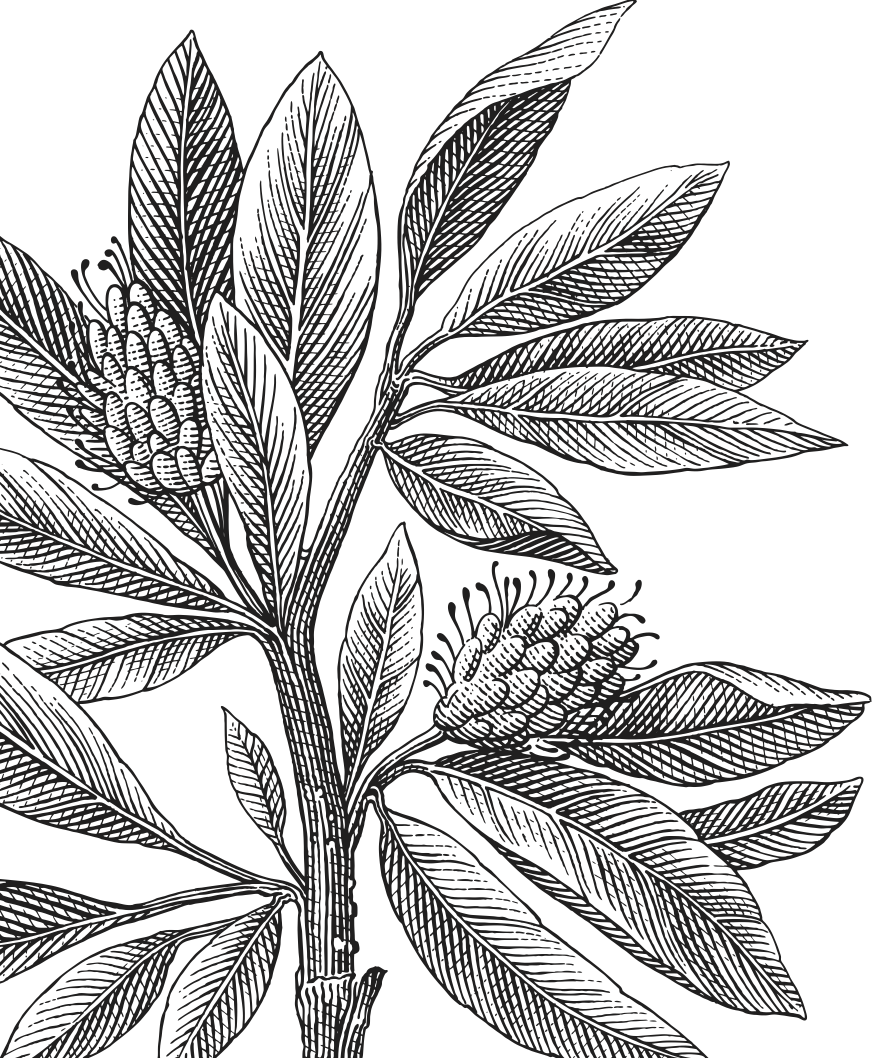
\includegraphics[keepaspectratio,scale=0.3]{lnu_etch.png} 
    }
}
\newcommand\BackgroundPicLogo{
    \put(30,740){
	
\includegraphics[keepaspectratio,scale=0.10]{logo.png}     
    }
}


\title{	
\vspace{-8cm}
\begin{sidebar}
    \vspace{5cm}
    \normalfont \normalsize
    \Huge Rapport \\
    \vspace{-1.3cm}
\end{sidebar}
\vspace{3cm}
\begin{flushleft}
    \huge Laboratory Report\\  
\end{flushleft}
\null
\vfill
\begin{textblock}{6}(10,13)
\begin{flushright}
\begin{minipage}{\textwidth}
\begin{flushleft} \large
	\emph{Author:} Caroline Nilsson \\ Daniel Alm Grundström \\
	%\emph{Handledare:} \\ 
	\emph{Termin:} HT 2017\\ 
	\emph{Course:} 1DT301 - Computer Technology I\\
\end{flushleft}
\end{minipage}
\end{flushright}
\end{textblock}
}
\date{\today} 



\begin{document}

\pagenumbering{gobble}
\newgeometry{left=5cm}
\AddToShipoutPicture*{\BackgroundPic}
\AddToShipoutPicture*{\BackgroundPicLogo}
\maketitle
\restoregeometry
\clearpage



\pagenumbering{gobble}

\tableofcontents
\newpage
\pagenumbering{arabic}



\section{Introduktion}
In the process of working with the laboratory assignments we started by doing research about the assembly language and the STK600 in order to better understand how to solve the different assignments. 
In each assignment we first created a pseudocode solution which we converted to flowchart diagrams, then it was rather simple to convert this into assembly language. Common for all assignments is also that we have been using the simulations to confirm that the program is working and completing the correct tasks. 

\newpage
\section{Assignment 1 - Light LED2}
In the first assignment we were to light up LED2 (which is the third light counting from the right). 

\begin{algorithm}
\begin{algorithmic}
\Procedure{Pseudocode}{}
\State{$PortB = output$}
\Repeat
\State{$Led2\ bitstring \rightarrow PortB$}
\Until{$\infty$}
\EndProcedure
\caption{Light LED2}
\label{assign1.pseudo}
\end{algorithmic}
\end{algorithm}

\begin{figure}[h]
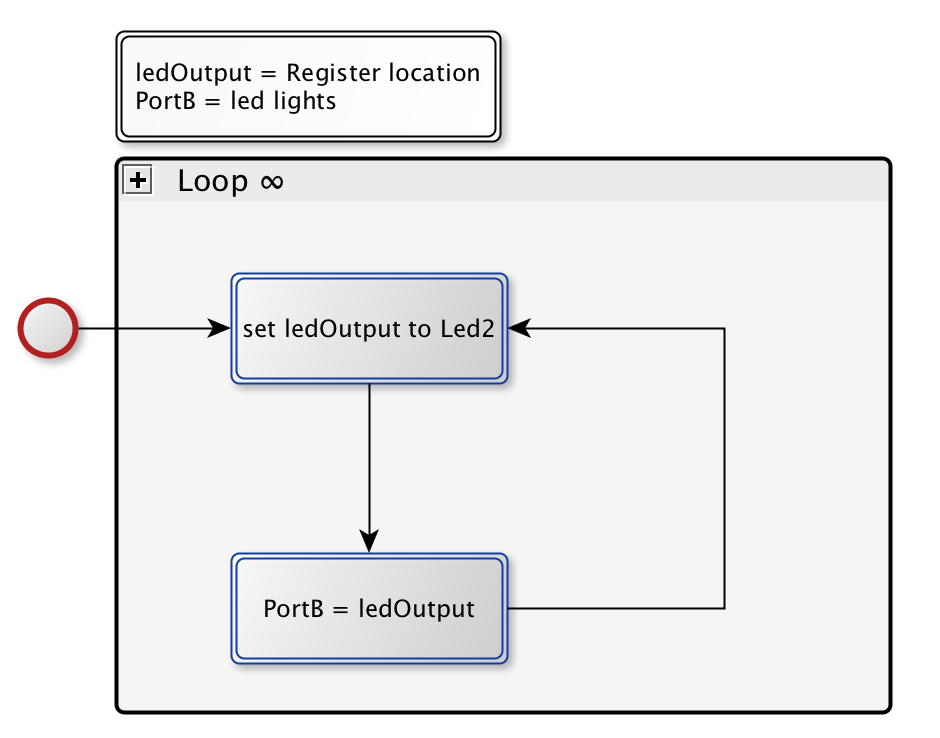
\includegraphics[scale=0.5]{Flowchart_pics/assignment1_pic.png} 
\caption{Flowchart}
\label{assign1.flow}
\end{figure}

The pseudocode (see algorithm \ref{assign1.pseudo}) and the flowchart (see figure \ref{assign1.flow}) shows that we first set Port B as an output port, the value 0000 0100 is saved at a register location (in our case that is R16) and then sent to Port B which makes LED2 (or the third led from the right) light up. 
Minimum lines of code?
\newpage
\subsection{Assembly Program}
\avrasm{../src/a1.asm}{}
\newpage

\section{Assignment 2 - Switch light corresponding LED}
\begin{algorithm}
\begin{algorithmic}
\Procedure{Pseudocode}{}
\State{$PortB = output$}
\State{$PortD = input$}
\Repeat
\State{$PortD\ value \rightarrow switchState$} \Comment{$switchState = register\ location$}
\State{$Invert\ value\ at\ switchState$}
\State{$switchState \rightarrow PortB$}
\Until{$\infty$}
\EndProcedure
\caption{Switches pressed lights corresponding LED}
\label{assign2.pseudo}
\end{algorithmic}
\end{algorithm}

\begin{figure}[h]
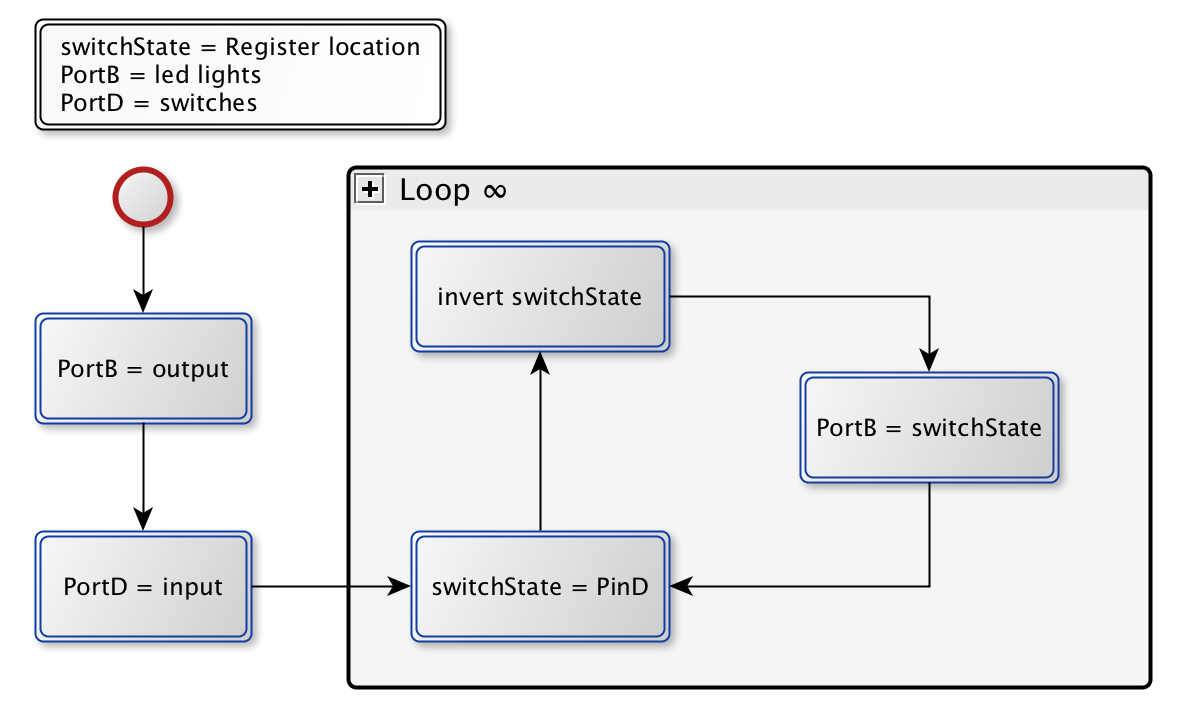
\includegraphics[scale=0.5]{Flowchart_pics/assignment2_pic.png} 
\caption{Basic flow in order to read switches and light corresponding LED}
\label{assign2.flow}
\end{figure}
\newpage
\subsection{Assembly Program}
\avrasm{../src/a2.asm}{}
\newpage

\section{Assignment 3 - Swift5 lights LED0}
\begin{algorithm}
\begin{algorithmic}
\Procedure{Pseudocode}{}
\State{$PortB = output$}
\State{$PortD = input$}
\Repeat
\State{$clear\ ledState$} \Comment{$ledState = register\ location$}
\If{$Switch5\ is\ pressed$}
\State{$ledState = LED0\ bit\ string$}
\EndIf
\State{$ledState \rightarrow PortB$}
\Until{$\infty$}
\EndProcedure
\caption{Light LED0 when switch5 is pressed}
\label{assign2.pseudo}
\end{algorithmic}
\end{algorithm}

\begin{figure}[h]
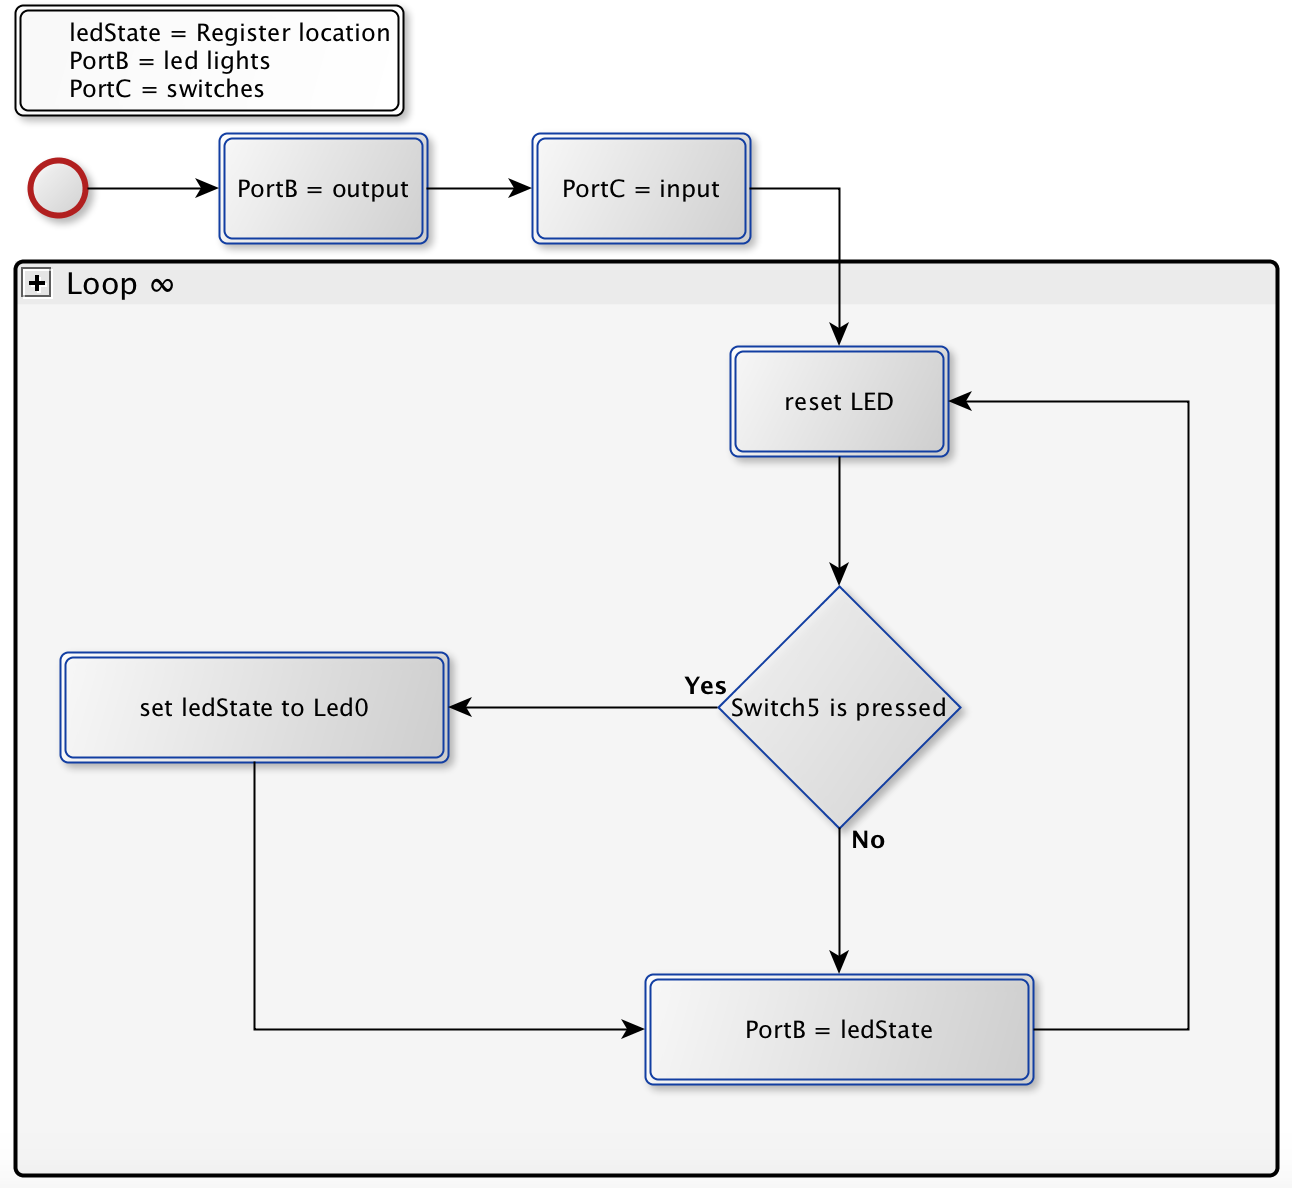
\includegraphics[scale=0.5]{Flowchart_pics/assignment3_pic.png} 
\caption{Flowchart}
\label{}
\end{figure}
\newpage
\subsection{Assembly Program}
\avrasm{../src/a3.asm}{}
\newpage

\section{Assignment 4}
\begin{algorithm}
\begin{algorithmic}
\Procedure{Pseudocode}{}
\State{}
\EndProcedure
\caption{}
\label{}
\end{algorithmic}
\end{algorithm}

\begin{figure}[h]

\caption{Flowchart}
\label{}
\end{figure}

\subsection{Assembly Program}
\begin{lstlisting}

\end{lstlisting}
\newpage

\section{Assignment 5 - Waterfall}
\begin{algorithm}
\begin{algorithmic}
\Procedure{Pseudocode}{}
\State{$Initialize\ stack\ pointer$}
\State{$PortB = output$}
\State{$ledState = 1$} \Comment{$ledState = register\ location$}
\Repeat
\State{$ledState \rightarrow PortB$}
\State{$Delay\ 0.5\ sec$}
\If{$LED7\ is\ lit$}
\State{$ledState = 1$}
\EndIf
\If{$LED7\ is\ not\ lit$}
\State{$Move\ to\ left$}
\EndIf
\Until{$\infty$}
\EndProcedure
\caption{Waterfall simulation using LEDs}
\label{}
\end{algorithmic}
\end{algorithm}

\begin{figure}[h]
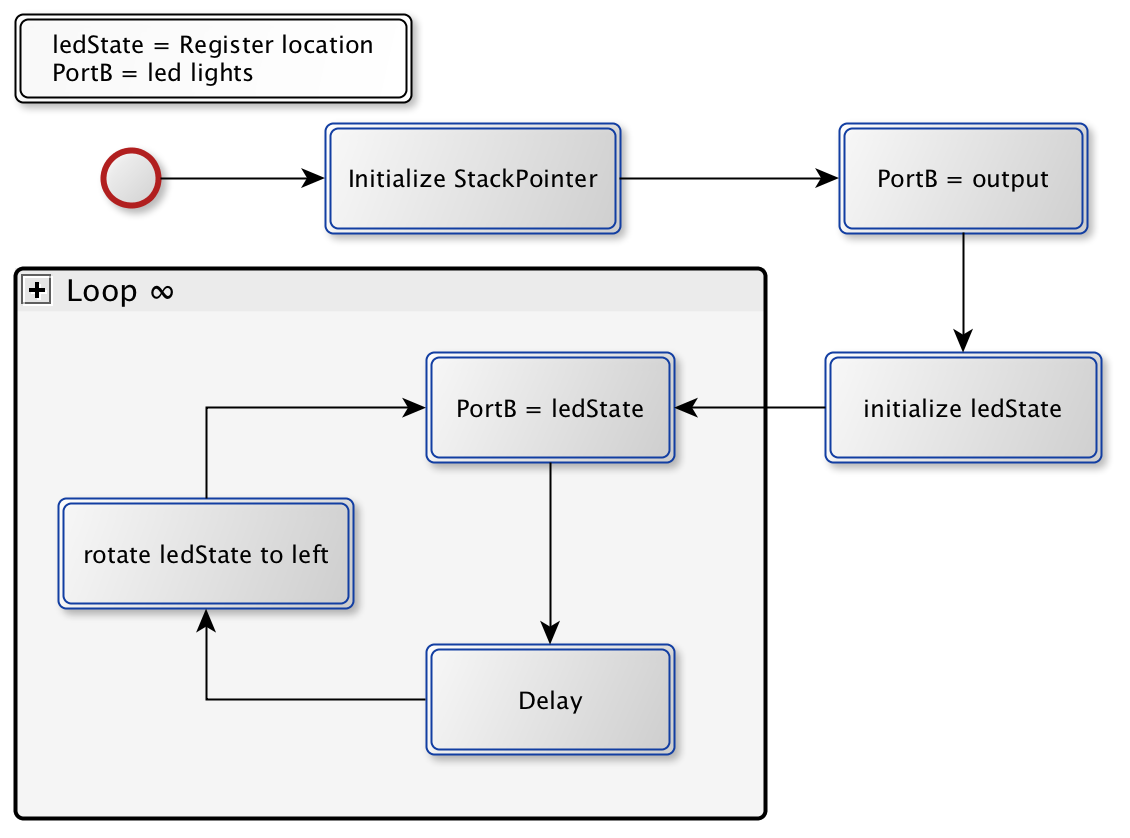
\includegraphics[scale=0.5]{Flowchart_pics/assignment5_pic.png} 
\caption{Flowchart}
\label{}
\end{figure}
\newpage
\subsection{Assembly Program}
\avrasm{../src/a5.asm}{}
\newpage

\section{Assignment 6 - Johnson counter}
\begin{algorithm}
\begin{algorithmic}
\Procedure{Pseudocode}{}
\State{$PortB = output$}
\State{$currentValue = 0$} \Comment{$currentValue = register\ location$}
\State{$multiplier = 2$} \Comment{$multiplier = register\ location$}
\Repeat \Comment{$Loop\_1\ (count\ up)$}
\If{$LED7\ is\ lit$}
\State{$Continue\ at\ Loop\_2$}
\Else
\State{$currentValue \times multiplier \rightarrow currentValue$}
\State{$Increase\ currentValue\ by\ 1$}
\EndIf
\State{$currentValue \rightarrow PortB$}
\State{$Delay\ 0.5\ sec$}
\Until{$\infty$}
\Repeat \Comment{$Loop\_2\ (count\ down)$}
\If{$LED0\ is\ lit$}
\State{$Continue\ at\ Loop\_1$}
\Else
\State{$Move\ right$}
\EndIf
\State{$currentValue \rightarrow PortB$}
\Until{$\infty$}
\EndProcedure
\caption{Johnson counter simulation using LEDs}
\label{}
\end{algorithmic}
\end{algorithm}

\begin{figure}[h!]
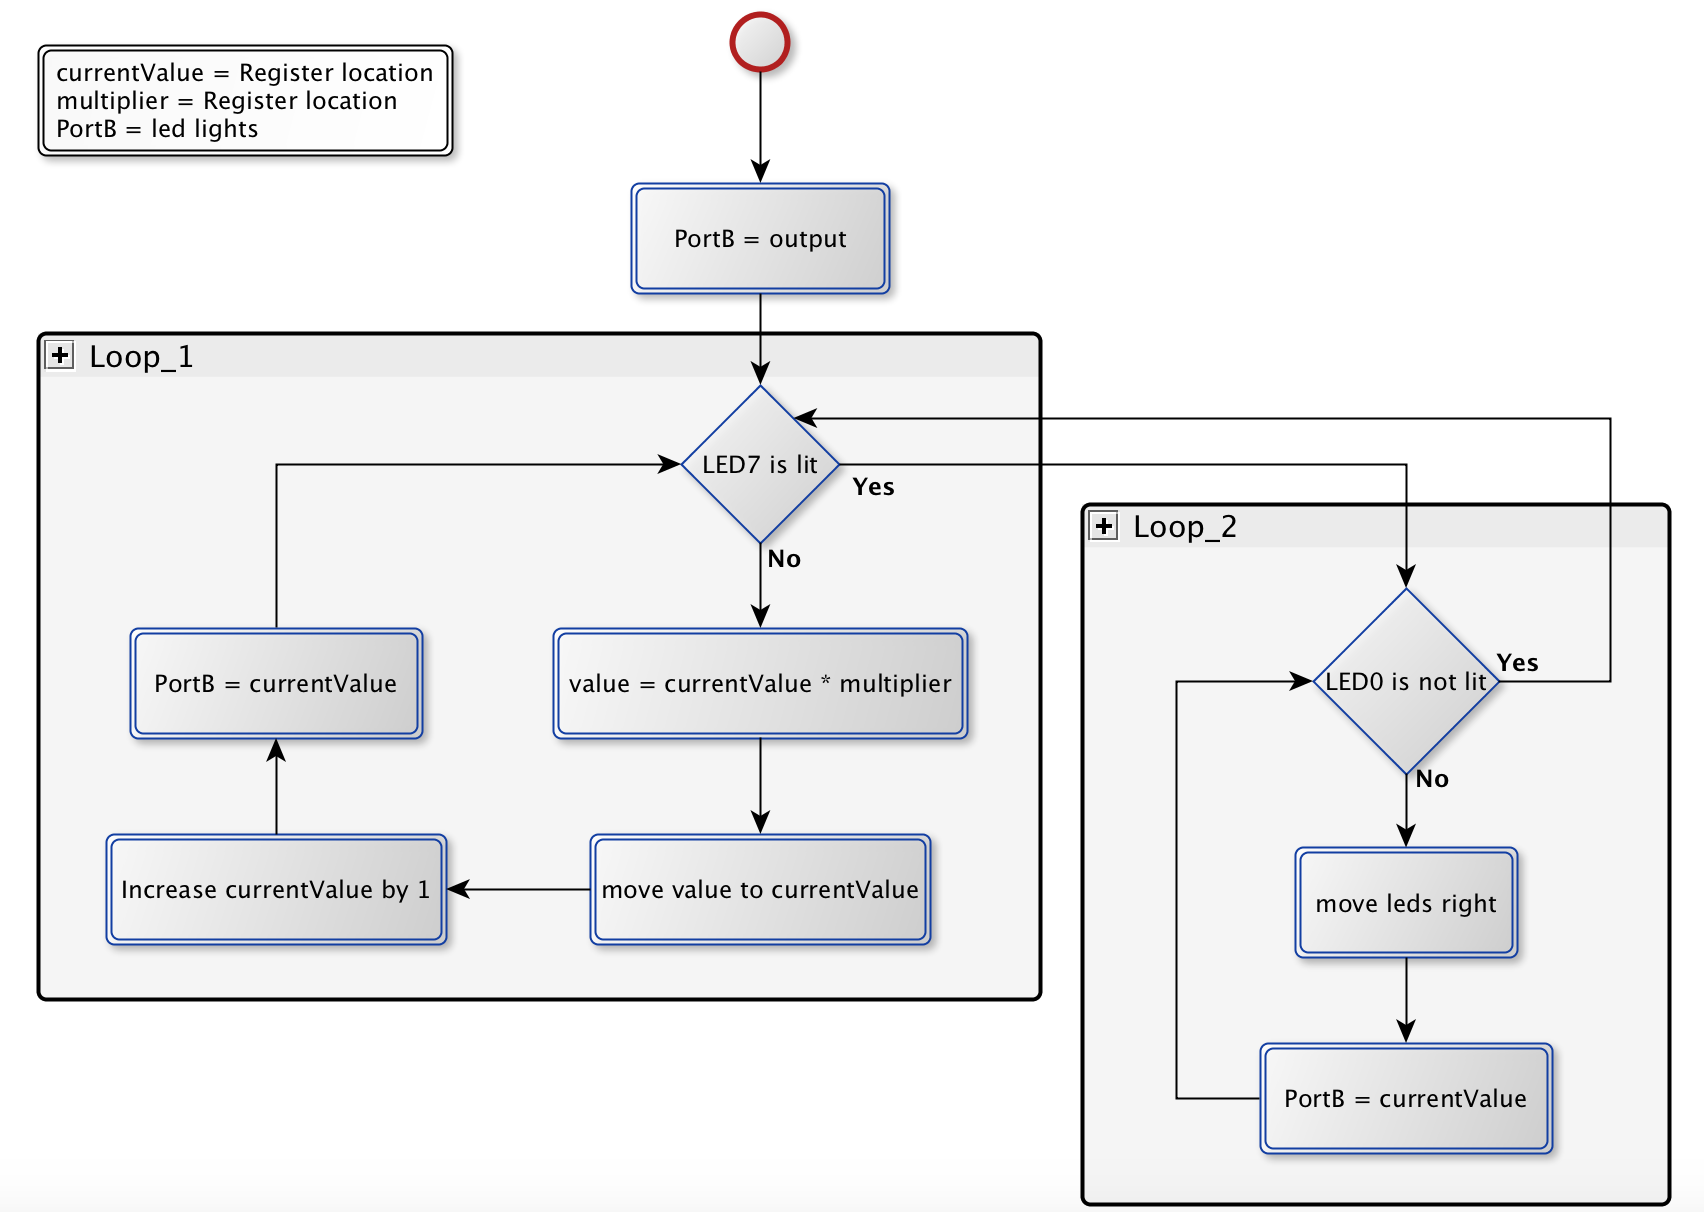
\includegraphics[scale=0.5]{Flowchart_pics/assignment6_pic.png} 
\caption{Flowchart}
\label{}
\end{figure}
\newpage
\subsection{Assembly Program}
\avrasm{../src/a6.asm}{}
\end{document}
